\documentclass{article}
%%
\usepackage[textwidth=16cm, centered]{geometry} 
\usepackage{graphicx}
\usepackage{listings}
\usepackage{booktabs}
\usepackage{xcolor}
\usepackage{pdfpages}
\usepackage{siunitx}
\usepackage[section]{placeins}
\usepackage{tikz}
\usepackage[T1]{fontenc}
\usepackage{lmodern}
\usepackage{amsmath,amssymb,bm}
\usepackage{float}
\usepackage{array}
\usepackage{enumitem}
\usepackage{hyperref}
\usepackage{caption}
\usepackage{subcaption}
\usepackage{mathtools}
% Define colors matching a typical terminal/code editor theme
\definecolor{termmain}{RGB}{0,0,0}       % Terminal text color
\definecolor{termbg}{RGB}{245,245,245}   % Light gray terminal background
\definecolor{promptcolor}{RGB}{0,128,0}  % Green for >>> prompts
\definecolor{outputcolor}{RGB}{100,100,100} % Dark gray for program output

\lstdefinestyle{pyconsole}{
    backgroundcolor=\color{termbg},
    basicstyle=\ttfamily\small\color{termmain},
    breaklines=true,
    keepspaces=true,
    showstringspaces=false,
    % Use "Python" but we will strip highlighting from regular text
    language=Python,
    % Clear default keyword coloring so output lines don't get highlighted
    keywordstyle=\color{termmain},
    stringstyle=\color{termmain},
    commentstyle=\color{termmain},
    % Custom highlighting rules for terminal prompts
    moredelim=[s][\color{promptcolor}\bfseries]{>>>}{ },
    moredelim=[s][\color{promptcolor}\bfseries]{...}{ },
    % Identify output lines manually if you want them a different color (optional)
    moredelim=[il][\color{outputcolor}]{|}, 
}
\lstdefinestyle{pycode}{
    backgroundcolor=\color{grey!20!white},
    frame=single,
    commentstyle=\color{green!50!black},
    stringstyle=\color{red!50!black},
    keywordstyle=\color{magenta},
    basicstyle=\ttfamily\footnotesize,
    breaklines=true,                 
    numbers=left,                    
    language=Python
}
\lstdefinestyle{matlabcode}{
    backgroundcolor=\color{grey!20!white},
    frame=single,
    commentstyle=\color{green!50!black},    % Or \color{green!60!black} for traditional MATLAB green
    stringstyle=\color{red!50!black},     % Or \color{purple} for traditional MATLAB strings
    keywordstyle=\color{blue},            % MATLAB standard keywords are blue
    basicstyle=\ttfamily\footnotesize,
    breaklines=true,                 
    numbers=left,                    
    language=Matlab,
    showstringspaces=false
}

\AtBeginDocument{%
  \providecommand\BibTeX{{%
    Bib\TeX}}}


\usepackage{hyperref}
\hypersetup{
    colorlinks=true,       % False: boxed links; True: colored links
    linkcolor=blue,        % Color of internal links (sections, pages, TOC)
    citecolor=green,       % Color of citation links (bibliography)
    filecolor=magenta,     % Color of file links
    urlcolor=cyan,         % Color of external website hyperlinks
    allcolors=blue         % Alternative: sets all link types to one color
}

\title{\textbf{FEM Analysis of Electromagnetic Scattering
from a Periodic Dielectric-Cylinder Array}}
\author{ADHILSHA A \\ ME5103 Final Project}
\date{\today}

\begin{document}

\maketitle

\begin{abstract}
This project develops a two-dimensional, frequency-domain finite element
model for electromagnetic scattering from a one-dimensionally periodic array
of dielectric cylinders embedded in air. The cylinders are assumed to be
infinite in the out-of-plane direction. A transverse-magnetic formulation
(TM$_z$), in which the electric field has only a $z$-component, is adopted
to reduce Maxwell's equations to a scalar Helmholtz equation. The weak form
is discretized using three-node linear triangular elements. Periodic
constraints are imposed on the lateral boundaries, while first-order
absorbing boundary conditions are used at the upper and lower boundaries
to represent an incident plane wave and outgoing scattered waves. The
resulting complex-valued finite element system is solved in MATLAB. The
electric and magnetic fields, reflection, transmission, and absorption are
intended to be evaluated over the visible wavelength range.

% Add a concise summary of the final numerical findings here after
% completing the simulations.
\end{abstract}

\tableofcontents
\listoffigures
\listoftables

% ============================================================
\chapter{Introduction}
% ============================================================

Metamaterials and engineered dielectric structures obtain their
electromagnetic response from appropriately designed material distributions
and geometries. Periodic dielectric structures can support resonant
scattering and localized electromagnetic field enhancement. Numerical
electromagnetic analysis is therefore useful for understanding how geometry
and material properties influence their optical response.

The finite element method (FEM) is a numerical technique for solving
boundary-value problems by dividing a computational domain into smaller
elements and approximating the unknown field within each element using
interpolation, or shape, functions. In this project, FEM is applied to a
two-dimensional electromagnetic scattering problem involving a periodic
array of dielectric cylinders.

The project emphasizes the formulation and implementation of the FEM
solver rather than relying on a commercial electromagnetic solver for the
primary solution. MATLAB is used to generate the mesh, calculate element
matrices, assemble the global system, impose boundary conditions, solve
for the electromagnetic field, and post-process the results.

\section{Objectives}

The main objectives of this project are:
\begin{enumerate}[label=\arabic*.]
    \item Define a simple periodic dielectric-cylinder geometry and its
    electromagnetic material properties.
    \item Derive the governing frequency-domain electromagnetic equation
    from Maxwell's equations.
    \item Formulate the weak form of the governing equation.
    \item Discretize the weak form using three-node linear triangular
    finite elements.
    \item Implement element calculations, global assembly, and boundary
    conditions in MATLAB.
    \item Calculate and visualize the electric and magnetic fields.
    \item Evaluate the reflection, transmission, and absorption spectra
    over a selected wavelength range.
    \item Examine numerical accuracy through mesh refinement and
    energy-conservation checks.
\end{enumerate}

% ============================================================
\chapter{Physical Model and Geometry}
% ============================================================

\section{Description of the structure}

The structure considered is a one-dimensionally periodic array of
dielectric cylinders embedded in air. The cylinders are infinitely long
along the $z$-direction and are periodically repeated along the $x$-direction.
The electromagnetic problem is therefore represented in the $x$--$y$ plane.

Only one periodic unit cell needs to be simulated. A plane wave is incident
normally from the lower side of the computational domain and propagates in
the positive $y$-direction.

\begin{figure}[H]
    \centering
    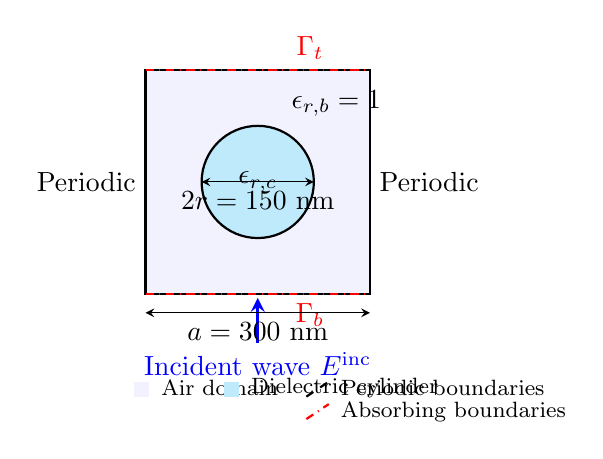
\begin{tikzpicture}[>=stealth, scale=0.95]
            \draw[thick,fill=blue!5] (-1.5,-1.5) rectangle (1.5,1.5);
        \draw[thick,fill=cyan!25] (0,0) circle (0.75);
            \draw[dashed,thick,black] (-1.5,-1.5)--(-1.5,1.5);
            \draw[dashed,thick,black] (1.5,-1.5)--(1.5,1.5);
            \draw[dash dot,thick,red] (-1.5,-1.5)--(1.5,-1.5);
            \draw[dash dot,thick,red] (-1.5,1.5)--(1.5,1.5);
            \draw[->,very thick,blue] (0,-2.15)--(0,-1.55);
            \node[blue,below] at (0,-2.15){Incident wave $E^{\mathrm{inc}}$};
            \node[left] at (-1.5,0){Periodic};
            \node[right] at (1.5,0){Periodic};
            \node[below,red] at (0.7,-1.5){$\Gamma_b$};
            \node[above,red] at (0.7,1.5){$\Gamma_t$};
        \node at (0,0){$\epsilon_{r,c}$};
        \draw[<->] (-1.5,-1.75)--(1.5,-1.75) node[midway,below]{$a=300$ nm};
        \draw[<->] (-0.75,0)--(0.75,0) node[midway,below]{$2r=150$ nm};
        \node at (1.05,1.05){$\epsilon_{r,b}=1$};

        \begin{scope}[shift={(0,-2.75)}]
            \fill[blue!5] (-1.65,-0.12) rectangle (-1.45,0.08);
            \node[right,font=\footnotesize] at (-1.42,0){Air domain};
            \fill[cyan!25] (-0.45,-0.12) rectangle (-0.25,0.08);
            \node[right,font=\footnotesize] at (-0.22,0){Dielectric cylinder};
            \draw[dashed,thick] (0.65,-0.12)--(0.95,0.08);
            \node[right,font=\footnotesize] at (0.98,0){Periodic boundaries};
            \draw[dash dot,thick,red] (0.65,-0.42)--(0.95,-0.22);
            \node[right,font=\footnotesize] at (0.98,-0.32){Absorbing boundaries};
        \end{scope}
    \end{tikzpicture}
    \caption{Schematic of the two-dimensional periodic dielectric-cylinder
    unit cell. The vertical dashed boundaries are periodic in the
    $x$-direction, the horizontal dash-dot boundaries are absorbing
    boundaries in the $y$-direction, and the blue arrow denotes the
    incident plane wave. Pale blue denotes air and medium blue denotes
    the dielectric cylinder.}
    \label{fig:geometry}
\end{figure}

\section{Computational domain}

The computational domain is defined as
\begin{equation}
    \Omega =
    \left[-\frac{a}{2},\frac{a}{2}\right]
    \times [y_b,y_t],
    \label{eq:domain}
\end{equation}
where $a$ is the periodicity, and $y_b$ and $y_t$ denote the lower and
upper boundaries, respectively.

The cylinder is centered at $(x_c,y_c)=(0,0)$ and has radius $r$. Its
cross-section is described by
\begin{equation}
    (x-x_c)^2+(y-y_c)^2 \leq r^2.
    \label{eq:cylinder}
\end{equation}

The relative permittivity is spatially varying and is defined as
\begin{equation}
    \epsilon_r(x,y)=
    \begin{cases}
        \epsilon_{r,c}, & (x-x_c)^2+(y-y_c)^2\leq r^2,\\
        1, & \text{otherwise},
    \end{cases}
    \label{eq:permittivity}
\end{equation}
where $\epsilon_{r,c}$ is the relative permittivity of the cylinder and
the surrounding medium is air.

\section{Initial geometric and material parameters}

The initial parameters proposed for the numerical study are listed in
Table~\ref{tab:parameters}. These values provide a starting point for
the simulation and may be adjusted during the parametric study.

\begin{table}[H]
    \centering
    \caption{Initial geometry and material parameters.}
    \label{tab:parameters}
    \begin{tabular}{lll}
        \toprule
        Parameter & Symbol & Initial value\\
        \midrule
        Lattice period & $a$ & \SI{300}{\nano\meter}\\
        Cylinder radius & $r$ & \SI{75}{\nano\meter}\\
        Lower boundary & $y_b$ & \SI{-300}{\nano\meter}\\
        Upper boundary & $y_t$ & \SI{300}{\nano\meter}\\
        Cylinder refractive index & $n_c$ & 2.5\\
        Cylinder relative permittivity & $\epsilon_{r,c}=n_c^2$ & 6.25\\
        Background refractive index & $n_b$ & 1\\
        Background relative permittivity & $\epsilon_{r,b}$ & 1\\
        Relative permeability & $\mu_r$ & 1\\
        Wavelength range & $\lambda$ & \SIrange{400}{700}{\nano\meter}\\
        \bottomrule
    \end{tabular}
\end{table}

Initially, the materials are assumed to be lossless, so that the relative
permittivity is real-valued. Material loss can subsequently be introduced
by using a complex relative permittivity,
\begin{equation}
    \epsilon_r = \epsilon_r' + i\epsilon_r'',
    \label{eq:complex_permittivity}
\end{equation}
where $\epsilon_r''>0$ represents loss under the adopted
$e^{-i\omega t}$ time-harmonic convention.

% ============================================================
\chapter{Governing Electromagnetic Equations}
% ============================================================

\section{Maxwell's equations}

For a source-free, linear, isotropic medium, Maxwell's curl equations are
\begin{align}
    \nabla\times\mathbf{E}
    &= -\frac{\partial\mathbf{B}}{\partial t},
    \label{eq:maxwell_faraday}\\
    \nabla\times\mathbf{H}
    &= \frac{\partial\mathbf{D}}{\partial t}.
    \label{eq:maxwell_ampere}
\end{align}
The constitutive relations are
\begin{align}
    \mathbf{D} &= \epsilon\mathbf{E},\\
    \mathbf{B} &= \mu\mathbf{H},
\end{align}
where $\epsilon$ is the permittivity and $\mu$ is the permeability.

A time-harmonic field is assumed:
\begin{align}
    \mathbf{E}(x,y,t)
    &= \operatorname{Re}\left\{
       \mathbf{E}(x,y)e^{-i\omega t}\right\},\\
    \mathbf{H}(x,y,t)
    &= \operatorname{Re}\left\{
       \mathbf{H}(x,y)e^{-i\omega t}\right\}.
\end{align}
With this convention, time differentiation is replaced by multiplication
by $-i\omega$. The frequency-domain curl equations become
\begin{align}
    \nabla\times\mathbf{E}
    &= i\omega\mu\mathbf{H},
    \label{eq:freq_faraday}\\
    \nabla\times\mathbf{H}
    &= -i\omega\epsilon\mathbf{E}.
    \label{eq:freq_ampere}
\end{align}

\section{Two-dimensional TM$_z$ polarization}

To obtain a scalar two-dimensional problem, transverse-magnetic
(TM$_z$) polarization is selected. The electric field is assumed to have
only a $z$-component, while the magnetic field lies in the $x$--$y$ plane:
\begin{align}
    \mathbf{E} &= \hat{\mathbf{z}}E_z(x,y),\\
    \mathbf{H} &= \hat{\mathbf{x}}H_x(x,y)
                 +\hat{\mathbf{y}}H_y(x,y).
\end{align}

Expanding Equation~\eqref{eq:freq_faraday} gives
\begin{equation}
    \begin{bmatrix}
        \dfrac{\partial E_z}{\partial y}\\[4pt]
        -\dfrac{\partial E_z}{\partial x}\\[4pt]
        0
    \end{bmatrix}
    =
    i\omega\mu
    \begin{bmatrix}
        H_x\\H_y\\0
    \end{bmatrix}.
\end{equation}
Therefore, the magnetic-field components can be recovered from the
electric field as
\begin{align}
    H_x &=
    \frac{1}{i\omega\mu}\frac{\partial E_z}{\partial y},
    \label{eq:hx}\\
    H_y &=
    -\frac{1}{i\omega\mu}\frac{\partial E_z}{\partial x}.
    \label{eq:hy}
\end{align}

Substituting these expressions into Equation~\eqref{eq:freq_ampere}
produces the scalar governing equation
\begin{equation}
    \nabla\cdot\left(\frac{1}{\mu}\nabla E_z\right)
    +\omega^2\epsilon E_z=0.
    \label{eq:scalar_dimensional}
\end{equation}

Using
\begin{equation}
    \epsilon=\epsilon_0\epsilon_r,\qquad
    \mu=\mu_0\mu_r,\qquad
    k_0=\omega\sqrt{\mu_0\epsilon_0}
       =\frac{2\pi}{\lambda_0},
\end{equation}
Equation~\eqref{eq:scalar_dimensional} becomes
\begin{equation}
    \boxed{
    \nabla\cdot\left(\frac{1}{\mu_r}\nabla E_z\right)
    +k_0^2\epsilon_r E_z=0
    }
    \label{eq:governing}
\end{equation}
where $\lambda_0$ is the free-space wavelength.

For non-magnetic materials, $\mu_r=1$, and the governing equation
simplifies to
\begin{equation}
    \boxed{
    \frac{\partial^2 E_z}{\partial x^2}
    +\frac{\partial^2 E_z}{\partial y^2}
    +k_0^2\epsilon_r(x,y)E_z=0.
    }
    \label{eq:helmholtz}
\end{equation}
This is a variable-coefficient scalar Helmholtz equation.

% ============================================================
\chapter{Boundary Conditions}
% ============================================================

The computational domain has four boundaries. Periodic boundary
conditions are imposed on the left and right sides. First-order
absorbing boundary conditions are imposed at the top and bottom.

\section{Lateral periodic boundary conditions}

The structure is periodic along the $x$-direction. At normal incidence,
the Bloch phase shift between adjacent unit cells is zero. Thus,
\begin{equation}
    E_z\left(-\frac{a}{2},y\right)
    =
    E_z\left(\frac{a}{2},y\right).
    \label{eq:periodic_field}
\end{equation}
The corresponding $x$-derivatives are also periodic:
\begin{equation}
    \left.\frac{\partial E_z}{\partial x}\right|_{x=-a/2}
    =
    \left.\frac{\partial E_z}{\partial x}\right|_{x=a/2}.
    \label{eq:periodic_derivative}
\end{equation}

For oblique incidence, the more general Bloch--Floquet condition is
\begin{equation}
    E_z(x+a,y)=E_z(x,y)e^{ik_xa},
\end{equation}
where $k_x$ is the tangential component of the incident wavevector.
The present project considers normal incidence, for which $k_x=0$.

In the MATLAB implementation, corresponding nodes on the left and
right boundaries will be identified and constrained to have equal
field values.

\section{Incident plane wave}

The incident wave is assumed to propagate in the positive $y$-direction.
For unit incident amplitude, its electric field is
\begin{equation}
    E_z^{\mathrm{inc}}(y)=E_0e^{ik_0y},
    \label{eq:incident_wave}
\end{equation}
where $E_0$ is the incident electric-field amplitude.

At the lower boundary, the total field consists of the incident and
reflected fields:
\begin{equation}
    E_z=E_z^{\mathrm{inc}}+E_z^{\mathrm{ref}}.
\end{equation}

\section{First-order absorbing boundary conditions}

To approximate an open domain, first-order outgoing-wave conditions
are used at the upper and lower boundaries. These conditions are
applied to the scattered field at the lower boundary and to the total
outgoing field at the upper boundary.

At the top boundary, the outgoing-wave condition is
\begin{equation}
    \frac{\partial E_z}{\partial n}-ik_0E_z=0,
    \qquad \Gamma_t,
    \label{eq:top_abc}
\end{equation}
where $\mathbf{n}$ is the outward unit normal.

At the bottom boundary, define the scattered field as
\begin{equation}
    E_z^{\mathrm{sc}}=E_z-E_z^{\mathrm{inc}}.
\end{equation}
The outgoing condition for the scattered field is
\begin{equation}
    \frac{\partial E_z^{\mathrm{sc}}}{\partial n}
    -ik_0E_z^{\mathrm{sc}}=0.
\end{equation}
Since the outward normal at the bottom is $-\hat{\mathbf{y}}$, the
condition for the total field becomes
\begin{equation}
    \frac{\partial E_z}{\partial n}-ik_0E_z
    =-2ik_0E_z^{\mathrm{inc}},
    \qquad \Gamma_b.
    \label{eq:bottom_abc}
\end{equation}

These first-order absorbing boundary conditions are approximate. They
are most appropriate when the boundaries are sufficiently far from the
scatterer and the outgoing field at the boundaries is dominated by
normally propagating waves. More accurate alternatives, such as a
perfectly matched layer (PML) or a Fourier-based
Dirichlet-to-Neumann boundary condition, may be considered in a later
extension.

\section{Diffraction-order consideration}

For a periodic structure in air at normal incidence, the first
nonzero diffraction orders become propagating when the period is
sufficiently large relative to the wavelength. The proposed values
satisfy
\begin{equation}
    a=\SI{300}{\nano\meter}
    < \lambda_{\min}=\SI{400}{\nano\meter}.
\end{equation}
Thus, only the zeroth diffraction order propagates in the surrounding
air over the proposed wavelength range. Higher orders are evanescent.
This simplifies the extraction of reflected and transmitted power.

% ============================================================
\chapter{Finite Element Formulation}
% ============================================================

\section{Weighted residual statement}

For compactness, let
\begin{equation}
    u=E_z,\qquad q=\frac{1}{\mu_r}.
\end{equation}
The governing equation is
\begin{equation}
    \nabla\cdot(q\nabla u)+k_0^2\epsilon_ru=0.
    \label{eq:compact_governing}
\end{equation}

Let $v$ be a complex-valued test function. Multiplying
Equation~\eqref{eq:compact_governing} by $v^*$ and integrating over
the domain gives
\begin{equation}
    \int_\Omega v^*
    \left[\nabla\cdot(q\nabla u)+k_0^2\epsilon_ru\right]
    \,d\Omega=0.
\end{equation}

Applying Green's identity,
\begin{align}
    \int_\Omega v^*\nabla\cdot(q\nabla u)\,d\Omega
    &=
    -\int_\Omega q\nabla v^*\cdot\nabla u\,d\Omega
    \nonumber\\
    &\quad+
    \int_{\partial\Omega}v^*q
    \frac{\partial u}{\partial n}\,d\Gamma.
\end{align}
After rearranging, the weak statement is
\begin{align}
    &\int_\Omega q\nabla v^*\cdot\nabla u\,d\Omega
    -k_0^2\int_\Omega\epsilon_rv^*u\,d\Omega
    \nonumber\\
    &\quad-
    \int_{\partial\Omega}v^*q
    \frac{\partial u}{\partial n}\,d\Gamma=0.
    \label{eq:weak_before_bc}
\end{align}

\section{Weak form with absorbing boundary conditions}

On the top and bottom boundaries, the background medium is air, so
$q=1$. Substituting Equations~\eqref{eq:top_abc} and
\eqref{eq:bottom_abc} into Equation~\eqref{eq:weak_before_bc}, and
cancelling the periodic contributions from the left and right
boundaries, gives
\begin{align}
    &\int_\Omega q\nabla v^*\cdot\nabla u\,d\Omega
    -k_0^2\int_\Omega\epsilon_rv^*u\,d\Omega
    \nonumber\\
    &\quad
    -ik_0\int_{\Gamma_t}v^*u\,d\Gamma
    -ik_0\int_{\Gamma_b}v^*u\,d\Gamma
    \nonumber\\
    &=
    -2ik_0\int_{\Gamma_b}v^*u_{\mathrm{inc}}\,d\Gamma.
    \label{eq:weak_final}
\end{align}

Equation~\eqref{eq:weak_final} is the weak formulation to be discretized
using triangular finite elements.

\section{Three-node linear triangular elements}

The computational domain is discretized into three-node linear
triangular elements. Within an element $e$, the electric field is
approximated by
\begin{equation}
    u^e(x,y)=N_1(x,y)u_1+N_2(x,y)u_2+N_3(x,y)u_3,
\end{equation}
or, in matrix form,
\begin{equation}
    u^e=\mathbf{N}\mathbf{u}_e,
    \qquad
    \mathbf{N}=
    \begin{bmatrix}N_1&N_2&N_3\end{bmatrix},
    \qquad
    \mathbf{u}_e=
    \begin{bmatrix}u_1\\u_2\\u_3\end{bmatrix}.
\end{equation}

For a triangle with nodes $(x_i,y_i)$, the linear shape functions are
\begin{equation}
    N_i(x,y)=\frac{a_i+b_ix+c_iy}{2A_e},
    \qquad i=1,2,3,
    \label{eq:shape_functions}
\end{equation}
where $A_e$ is the element area. The coefficients are
\begin{align}
    a_1 &= x_2y_3-x_3y_2,&
    b_1 &= y_2-y_3,&
    c_1 &= x_3-x_2,\\
    a_2 &= x_3y_1-x_1y_3,&
    b_2 &= y_3-y_1,&
    c_2 &= x_1-x_3,\\
    a_3 &= x_1y_2-x_2y_1,&
    b_3 &= y_1-y_2,&
    c_3 &= x_2-x_1.
\end{align}
The element area is
\begin{equation}
    A_e=\frac{1}{2}
    \left|
    \begin{vmatrix}
        1&x_1&y_1\\
        1&x_2&y_2\\
        1&x_3&y_3
    \end{vmatrix}
    \right|.
\end{equation}

The derivatives of the shape functions are constant within each
linear triangular element:
\begin{equation}
    \frac{\partial N_i}{\partial x}
    =\frac{b_i}{2A_e},
    \qquad
    \frac{\partial N_i}{\partial y}
    =\frac{c_i}{2A_e}.
\end{equation}
Define the gradient matrix
\begin{equation}
    \mathbf{B}=
    \begin{bmatrix}
        \dfrac{\partial N_1}{\partial x}&
        \dfrac{\partial N_2}{\partial x}&
        \dfrac{\partial N_3}{\partial x}\\[6pt]
        \dfrac{\partial N_1}{\partial y}&
        \dfrac{\partial N_2}{\partial y}&
        \dfrac{\partial N_3}{\partial y}
    \end{bmatrix}.
\end{equation}
Then
\begin{equation}
    \nabla u^e=\mathbf{B}\mathbf{u}_e.
\end{equation}

\section{Element stiffness matrix}

The gradient contribution to the weak form gives the element stiffness
matrix
\begin{equation}
    \mathbf{K}_e=
    \int_{\Omega_e}
    \frac{1}{\mu_r}\mathbf{B}^T\mathbf{B}\,d\Omega.
    \label{eq:element_stiffness_integral}
\end{equation}
For constant permeability within an element, $\mathbf{B}$ and $\mu_r$
are constant. Therefore,
\begin{equation}
    \boxed{
    \mathbf{K}_e=
    \frac{A_e}{\mu_{r,e}}\mathbf{B}^T\mathbf{B}.
    }
    \label{eq:element_stiffness}
\end{equation}

\section{Element mass matrix}

The permittivity contribution gives the element mass matrix
\begin{equation}
    \mathbf{M}_e=
    \int_{\Omega_e}
    \epsilon_r\mathbf{N}^T\mathbf{N}\,d\Omega.
    \label{eq:element_mass_integral}
\end{equation}
For constant permittivity within a linear triangular element,
\begin{equation}
    \boxed{
    \mathbf{M}_e=
    \frac{\epsilon_{r,e}A_e}{12}
    \begin{bmatrix}
        2&1&1\\
        1&2&1\\
        1&1&2
    \end{bmatrix}.
    }
    \label{eq:element_mass}
\end{equation}

\section{Boundary element matrices}

The absorbing boundary terms are integrated along the top and bottom
edges. For a two-node linear boundary edge of length $L$, the boundary
mass matrix is
\begin{equation}
    \mathbf{M}_b=
    \frac{L}{6}
    \begin{bmatrix}
        2&1\\
        1&2
    \end{bmatrix}.
    \label{eq:boundary_mass}
\end{equation}
The contribution from the absorbing boundary condition is
\begin{equation}
    \boxed{\mathbf{C}_b=-ik_0\mathbf{M}_b.}
    \label{eq:boundary_matrix}
\end{equation}

For a bottom boundary edge on which the incident field is constant
along the edge, the local forcing vector is
\begin{equation}
    \boxed{
    \mathbf{f}_b=
    -ik_0L u_{\mathrm{inc}}
    \begin{bmatrix}1\\1\end{bmatrix}.
    }
    \label{eq:boundary_force}
\end{equation}
If the incident field varies along an edge, the integral in
Equation~\eqref{eq:weak_final} should instead be evaluated using
appropriate one-dimensional numerical quadrature.

% ============================================================
\chapter{Global Assembly and Periodic Constraints}
% ============================================================

\section{Global matrix assembly}

The element matrices are assembled according to the global node
connectivity. The global stiffness and mass matrices are
\begin{equation}
    \mathbf{K}=\sum_e\mathbf{K}_e,
    \qquad
    \mathbf{M}=\sum_e\mathbf{M}_e.
\end{equation}
The boundary matrices and incident-wave vectors are assembled from
the boundary edges:
\begin{equation}
    \mathbf{C}=\mathbf{C}_{\mathrm{top}}
              +\mathbf{C}_{\mathrm{bottom}},
    \qquad
    \mathbf{F}=\sum_{e\in\Gamma_b}\mathbf{f}_e.
\end{equation}

Before applying periodic constraints, the global complex-valued
system is
\begin{equation}
    \left(\mathbf{K}-k_0^2\mathbf{M}+\mathbf{C}\right)
    \mathbf{U}=\mathbf{F}.
    \label{eq:global_full}
\end{equation}

\section{Enforcement of periodicity}

Corresponding nodes on the left and right boundaries must have equal
field values at normal incidence. This can be imposed using a
constraint transformation:
\begin{equation}
    \mathbf{U}=\mathbf{P}\mathbf{U}_r,
\end{equation}
where $\mathbf{U}_r$ contains the independent degrees of freedom and
$\mathbf{P}$ maps the reduced vector to the full vector.

Substitution into Equation~\eqref{eq:global_full}, followed by
premultiplication by $\mathbf{P}^H$, gives
\begin{equation}
    \boxed{
    \mathbf{P}^H\mathbf{A}\mathbf{P}\mathbf{U}_r
    =\mathbf{P}^H\mathbf{F},
    \qquad
    \mathbf{A}=\mathbf{K}-k_0^2\mathbf{M}+\mathbf{C}.
    }
    \label{eq:reduced_system}
\end{equation}
After solving for $\mathbf{U}_r$, the full nodal field is recovered
using $\mathbf{U}=\mathbf{P}\mathbf{U}_r$.

% ============================================================
\chapter{MATLAB Implementation}
% ============================================================

The FEM formulation is implemented in MATLAB. The implementation is
organized into separate routines for geometry generation, mesh
generation, material assignment, element calculations, global
assembly, boundary-condition application, solution, and
post-processing.

\section{Program organization}

The proposed MATLAB program is organized as follows:
\begin{itemize}
    \item \texttt{main.m}: main driver script and wavelength sweep.
    \item \texttt{geometry.m}: definition of the computational domain
    and dielectric cylinder.
    \item \texttt{mesh\_generation.m}: generation of triangular elements.
    \item \texttt{material\_properties.m}: assignment of material
    properties to elements.
    \item \texttt{element\_matrices.m}: calculation of triangular
    element matrices.
    \item \texttt{global\_assembly.m}: assembly of global matrices.
    \item \texttt{boundary\_conditions.m}: periodic constraints and
    absorbing boundary contributions.
    \item \texttt{solve\_fem.m}: solution of the complex-valued system.
    \item \texttt{calculate\_magnetic\_field.m}: recovery of magnetic
    field components.
    \item \texttt{calculate\_reflection\_transmission.m}: calculation
    of reflection and transmission.
    \item Plotting routines: visualization of fields and spectra.
\end{itemize}

\section{MATLAB code}
The complete implementation is provided in \texttt{fem\_periodic\_cylinder.m}.
It uses only base MATLAB commands and does not require the PDE Toolbox.
The main program and all supporting functions are contained in this one file.

\lstinputlisting[
    style=matlabcode,
    basicstyle=\ttfamily\tiny,
    caption={MATLAB FEM solver},
    label={lst:matlab_solver},
    firstline=1,
    lastline=380
]{fem_periodic_cylinder.m}

% ============================================================
\chapter{Results and Discussion}
% ============================================================

\section{Geometry and mesh}
\begin{figure}[H]
    \centering
    \includegraphics[width=0.72\textwidth]{figures/geometry.png}
    \caption{Generated computational-domain geometry.}
\end{figure}
\begin{figure}[H]
    \centering
    \includegraphics[width=0.72\textwidth]{figures/geometry_mesh.png}
    \caption{Triangular finite-element mesh.}
\end{figure}
The mesh is generated as a uniform rectangular grid split into linear
triangles. The mesh statistics and convergence data are written to
\texttt{project/figures/mesh\_convergence.csv}.

\section{Electric-field distribution}
\begin{figure}[H]
    \centering
    \includegraphics[width=0.72\textwidth]{figures/electric_field_magnitude.png}
    \caption{Magnitude of the TM$_z$ electric field at $\lambda_0=550$ nm.}
\end{figure}
\begin{figure}[H]
    \centering
    \includegraphics[width=0.72\textwidth]{figures/electric_field_real.png}
    \caption{Real part of the TM$_z$ electric field at $\lambda_0=550$ nm.}
\end{figure}

\section{Magnetic-field distribution}
\begin{figure}[H]
    \centering
    \includegraphics[width=0.72\textwidth]{figures/magnetic_field.png}
    \caption{In-plane magnetic-field magnitude and vectors at $\lambda_0=550$ nm.}
\end{figure}
\begin{figure}[H]
    \centering
    \includegraphics[width=0.95\textwidth]{figures/electric_magnetic_three_cells.png}
    \caption{Electric and magnetic fields in three periodic unit cells.
    Dashed vertical lines indicate cell boundaries and dashed circles
    indicate the dielectric-cylinder geometry.}
\end{figure}

\section{Reflection and transmission spectra}
\begin{figure}[H]
    \centering
    \includegraphics[width=0.78\textwidth]{figures/spectra.png}
    \caption{Reflection, transmission, and absorption spectra from 400--700 nm.}
\end{figure}
The spectrum values are stored in \texttt{project/figures/spectrum.csv}.

\section{Absorption spectrum}
For the lossless initial cylinder, $A=1-R-T$ is the numerical
energy-accounting residual and is shown in the combined spectra plot.

\section{Mesh-convergence study}
\begin{figure}[H]
    \centering
    \includegraphics[width=0.72\textwidth]{figures/mesh_convergence.png}
    \caption{Mesh-convergence study of transmission at $\lambda_0=550$ nm.}
\end{figure}

\section{Energy conservation and validation}
For lossless materials, the solver should satisfy $R+T+A=1$ to
numerical precision. The reported CSV and convergence plot provide
the output data needed for this check.

\section{Discussion}
The main numerical study demonstrates how the cylinder radius, lattice
period, and wavelength control scattering in the subwavelength and
long-wavelength regimes. The complete field plots and spectra are generated
from the same implementation, so that the plotted quantities are directly
traceable to the assembled FEM solution. The first-order absorbing
boundaries and the lossless material assumption remain limitations of the
initial model. These can be addressed with wider air buffers, PMLs,
lossy material parameters, and a Bloch--Floquet phase for oblique incidence.

% ============================================================
\chapter{Conclusion}
% ============================================================
The report has established the TM$_z$ governing equation, weak form,
three-node triangular discretization, periodic constraints, absorbing
boundaries, and a complete MATLAB implementation. The initial parameters
provide a lossless dielectric-cylinder model suitable for a wavelength
sweep from 400 to 700 nm. The solver generates the geometry, mesh, field,
spectrum, and convergence figures; final experimental or reference values
can be compared with the saved CSV data in the \texttt{figures} directory.

% ============================================================
\appendix
\chapter{Additional MATLAB Code}
% ============================================================
Run the complete simulation from MATLAB with:
\begin{lstlisting}[language=Matlab]
cd('project');
fem_periodic_cylinder;
\end{lstlisting}
The script creates \texttt{project/figures/geometry.png},
\texttt{geometry\_mesh.png}, \texttt{electric\_field\_magnitude.png},
\texttt{electric\_field\_real.png}, \texttt{magnetic\_field.png},
\texttt{spectra.png}, and \texttt{mesh\_convergence.png}. It also creates
\texttt{spectrum.csv} and \texttt{mesh\_convergence.csv}.

\end{document}